\section{Abstract}

Brain simulations are often used in neuroscience to test theoretical models of computation. Understanding the low-level dynamics of the brain is fundamental to develop better artificial intelligence algorithms, and in turn those algorithms provide more sophisticated methods to crack the brain code. 
Still, building simulations of sections of the brain is complex, and finding the parameters of the neurons and synapses so that the behavior of the artificial network matches the biological one requires a lot of time and resources.
Here it is developed a simple framework to automate the search for the best parameters for the simulation, and is provided a use case with a model of a hypercolumn and a Reinforcement Learning algorithm to optimize the parameters so that the firing rate of the excitatory populations in every layer matches the activity recorded in vivo.
The results show that Reinforcement Learning obtains results that exceed in accuracy the referenced papers.

\section{Theoretical Introduction}
\begin{quote}
``Computational Neuroscience is an approach to understanding the information content of neural signals by modeling the nervous system at many different structural scales, including the biophysical, the circuit, and the systems levels. Computer simulations of neurons and neural networks are complementary to traditional techniques in neuroscience.''
\begin{flushright}
\cite[Series Foreword]{dayan}
\end{flushright}
\end{quote}
Understanding how the brain works is one of the hardest challenges the humanity has ever faced, and it is crucial in the progress of Science: understanding intelligence, the learning process and consciousness would be groundbreaking for the developing of new technologies.

One of the main issues in the study of the brain right now is retrieving the data: we have enough computational power to process signals from billions of neurons at the same time, but we can't just put an electrode in everyone of them, although some are going in that direction \cite{neuralink}. 

There are other widely used technologies that are able to records brain metabolism or electromagnetic fields and currents over the scalp, and they can help to figure out correlation between high level cognitive functions and active brain areas, but they don't offer insights on low level computations. Cellular biology is very interested in synaptic transmission, and their research is inspiring Deep Learning researchers to try understand how the brain uses action potentials to carry information, and how the computations occur from a algorithmic point of view.

\myparagraph{Deep Learning and Neuroscience} 
Research in neuroscience has historically been driven by a biological approach: it has been focused on how the cells were structured, on how the genome influenced the production on neurotransmitters and how those neurotransmitters could shape behavior. 

Then, a movement, mostly inspired by physics, started interesting on circuits: how does the electromagnetic waves of lights become perception? How does we decide and control our movement in the space? Many instrumentation was developed to study the brain while on task, like EEG, MEG, PET and fMRI, but none of them could give us the same insight as the one given by invasive techniques such as in cell recordings. 

Lastly, around ten years ago \cite{lecun2015deep}, Deep Learning was rediscovered, thanks to the development of high parallel computing power (GPUs), and the real potential of artificial neural networks came to light. 

Deep Learning started having a profound impact on Neuroscience, not only thanks to the new methods that it carried for analyzing data and comparing circuits and their behaviours, but also for the change in objective: Cognitive and Computational Neuroscience was aimed to understand the brain and how it works, but the most prominent use cases were clinical. With Deep Learning, discovering a more efficient learning algorithm is worth billions of dollars and, like it or not, this influences research heavily.

Right now, understanding how the brain works, how the mind works, has the potential to exhibit new ways to make machines learn, to shed light on the most efficient ways to program an algorithm able to do what only living beings seem to do well: perceiving, orienteering, understanding language, producing language and ultimately reasoning.

The underlying hypotheses that sustain the research are a) that understanding how the brain solves computational challenges can help to build better algorithms and b) that better algorithms hopefully allows for a deeper comprehension of the brain. The developed algorithms will enable more efficient methods to study many areas, like computational biology \cite{angermueller2016deep}, traffic flow prediction \cite{koesdwiady2016improving}, improvement of existing techniques of brain imaging \cite{milletari2017hough}, financial market prediction \cite{fischer2018deep} and many more.

Although the perspective of a machine able to ``think'' is still very far away, research is obtaining incredible results with deep learning, and it isn't showing signs of a slow.

What is missing though, is a deeper connection between Neuroscience research and AI research. A recent paper \cite{richards2019deep} promotes this link, proposing to apply the AI framework to the study of Neuroscience, and pointing out that we absolutely need advances in the latter to proceed with the first.

In particular, understanding how brain connectivity is able to determine certain kinds of computations, is a topic of major interest in the field of Deep Learning, specifically to be able to design network's architectures that obtain high performance on the set of tasks that living beings excel at.

A use case is to compare an algorithm for a given task, like visual recognition, to the brain circuit that executes that task, in this case the ventral system of vision, to understand if there are similarities in the behavior and if they correlate with higher performance.

To do so it is necessary to record and understand how the system of interest works, how it is connected, and how it reacts to a stimulus. This can be very hard, because with the technologies available in this time this usually requires an invasive approach, so it can't be done on many humans. This is where simulations come into play: a simulation can help infer the internal dynamics of the given system without requiring full knowledge of it. 

Still, inference is usually computationally complex and non-linear, so finding the exact parameters for every neuron and every connection in a big model, while respecting the imposed thresholds and without full knowledge of the system is very challenging for an ordinary algorithm. 

\myparagraph{What is Deep Learning}
Deep Learning is a machine learning method, based on an extension of the \emph{perceptron} \cite{rosenblatt1958perceptron}, and can be used as classifier or to approximate functions. A Deep Learning architecture, a Deep Neural Network, is composed of nodes and links, where the former are characterized by an \emph{activation function}, and the latter by a weight, that usually is random first and is changed to optimize the outcome thanks to Stochastic Gradient Descent \cite{robbins1951stochastic} or an evolution of it. The nodes are organized in layers, and they can be fully connected or have convolutional or recursive features. The first layer is called ``input layer'', the last one ``output layer'' and the ones in between them are called ``hidden layers''. 
The input layer is a vector of nodes, and has the same shape of the data. The hidden layers can be of any size, and there can be as many as is wished. The size of the output layer is equal to the number of the classes, in the case of a classifier model, or equal to the output size of the function that it is intended to approximate.

The activation function is a nonlinear function, usually a Rectified Linear function for the nodes in the hidden layers and a specific function in the output layer, depending on the context. 
There are many parameters to be defined in a Deep Neural Network, but the more prominent are the learning rate, the depth and the activation functions.


\myparagraph{Simulations} 
A less invasive solution is to use our knowledge of the brain to build complex, biologically plausible simulations of the brain, or parts of the brain, and then retrieve from them all the data that is needed. This data can then be used to predict behaviors of real networks, to understand non-linear dynamics, or to test whether the understanding of a phenomena is accurate enough to provide all the information needed to reproduce it.

However, this approach, deeply analyzed in the past \cite{smolensky}, doesn't offer assurance that the simulation and the real process could actually be interchangeable. In the present, many of the challenges of that time were overcome, in particular computational power \cite{bluegene}, and simulations are used to confirm theoretical models of the brain.


\myparagraph{The Framework} 
Here is proposed a simple framework to guide the search for the parameters of a model of the brain, in an autonomous fashion and with high accuracy results. 

The elements of the framework are just the simulation model and the optimization algorithm, and they are characterized by the fixed and the free parameters for the simulation, while for the algorithm is featured by its loss function, so which output of the simulation is evaluated and how, its $k$ parameter, representing the scale of the output, and its structure.

In this study the simulation model, that will be described in more detail later, is an hypothetical column of the sensory cortex of a mammal, developed by Potjans \cite{potjans}, the free parameters are a subset of the ones they found to minimize the difference of the firing rate of the excitatory neurons in four different layers of the simulation between the firing rates of the respective population and layers in the in vivo situation. So the firing rate is the output of the simulation that is evaluated. The $k$ parameters will vary between different simulation to find the most adeguate for each case. Finally, the structure of the optimization algorithm will be derived from a Reinforcement Learning Algorithm, namely Deep Deterministic Policy Gradient (DDPG) \cite{lillicrap}, whose functioning will be explained in the next section.


\subsection{Reinforcement Learning} 


Reinforcement Learning is an area of machine learning which considers a setup consisting of an agent interacting with an environment through actions. The agent receives an input from the environment, chooses an action and receives a reward, based on the state of the environment after the action.

For example, the environment could be a model of a neuron connected to a spike detector, and the action at disposal of the agent could be to change the constant background current of the neuron. If its objective is to have the neuron spike with a specific rate, like 4 spikes per second, then the reward could be the absolute difference between the firing rate of the previous second and the one desired.

The agent would be rewarded less when it achieves a firing rate very different from 4 spikes per second, and more when it is close, so it will gradually learn to approach the right value.

This way of modeling the problem of learning is called \emph{Markov Decision Process}, and it provides a mathematical framework that let artificial agents make optimal decisions in a noisy environment where the agent has missing information about its internal dynamics.

Reinforcement Learning has shown the potential to understand highly complex observation spaces, as in the game of go \cite{silver2017mastering}, in videogame \cite{vinyals2019alphastar}, \cite{berner2019dota}, robotic control \cite{andrychowicz2020learning} and autonomous vehicles systems \cite{sallab2017deep}, but most importantly, it has been showed in some domains, such as predicting protein structure \cite{alphafold}, that Deep Reinforcement Learning is well suited to learn complex features of models and act to modify them in a desired direction.

\myparagraph{The actor-critic} 
DDPG belongs to the family of actor-critic algorithms, which use an action-value function (called the critic) to process the distribution of rewards over actions, and a policy (called the actor) to find the best possible action.

Actor-critic algorithms were developed to overcome the limitations of ``actor-only'' and ``critic-only'' algorithms, as stated in the paper that introduced them:

\begin{quote}
\begin{itemize}
	\item Actor-only methods work with a parameterized family of policies. The gradient of the performance, with respect to the actor parameters, is directly estimated by simulation, and the parameters are updated in a  direction of improvement. A possible drawback of such methods is that the gradient estimators may have a  large variance. Furthermore, as the policy changes, a  new gradient is estimated independently of past estimates. Hence, there is no ``learning,'' in the sense of accumulation and consolidation of older information. 

	\item Critic-only methods rely exclusively on value function approximation and aim at learning an approximate solution to the Bellman equation, which will then hopefully prescribe a  near-optimal policy. Such methods are indirect in the sense that they do not try to optimize directly over a policy space. A method of this type may succeed in constructing a ``good'' approximation of the value function, yet lack reliable guarantees in terms of near-optimality of the resulting policy.
\end{itemize}
	\begin{flushright}
		\cite{konda2000actor}	
	\end{flushright}
\end{quote}
The critic takes the value of an action and the reward obtained executing it and tries to shape a function that assigns to every action a value, called Q-value, that represent the expected reward after taking the action. The policy (the actor) defines the agent behavior, and its job is to take the present state as input and to choose an action.

To train the actor, DDPG uses the critic: in the previous example, the actor training process would be to take a set of actions in some random states, and then the critic would evaluate them, and the negative mean loss of the critic would be the loss of the actor. The actor and the critic are function approximation algorithms, in this case Artificial Neural Networks (ANNs).

\begin{figure}[h]
	\centering
	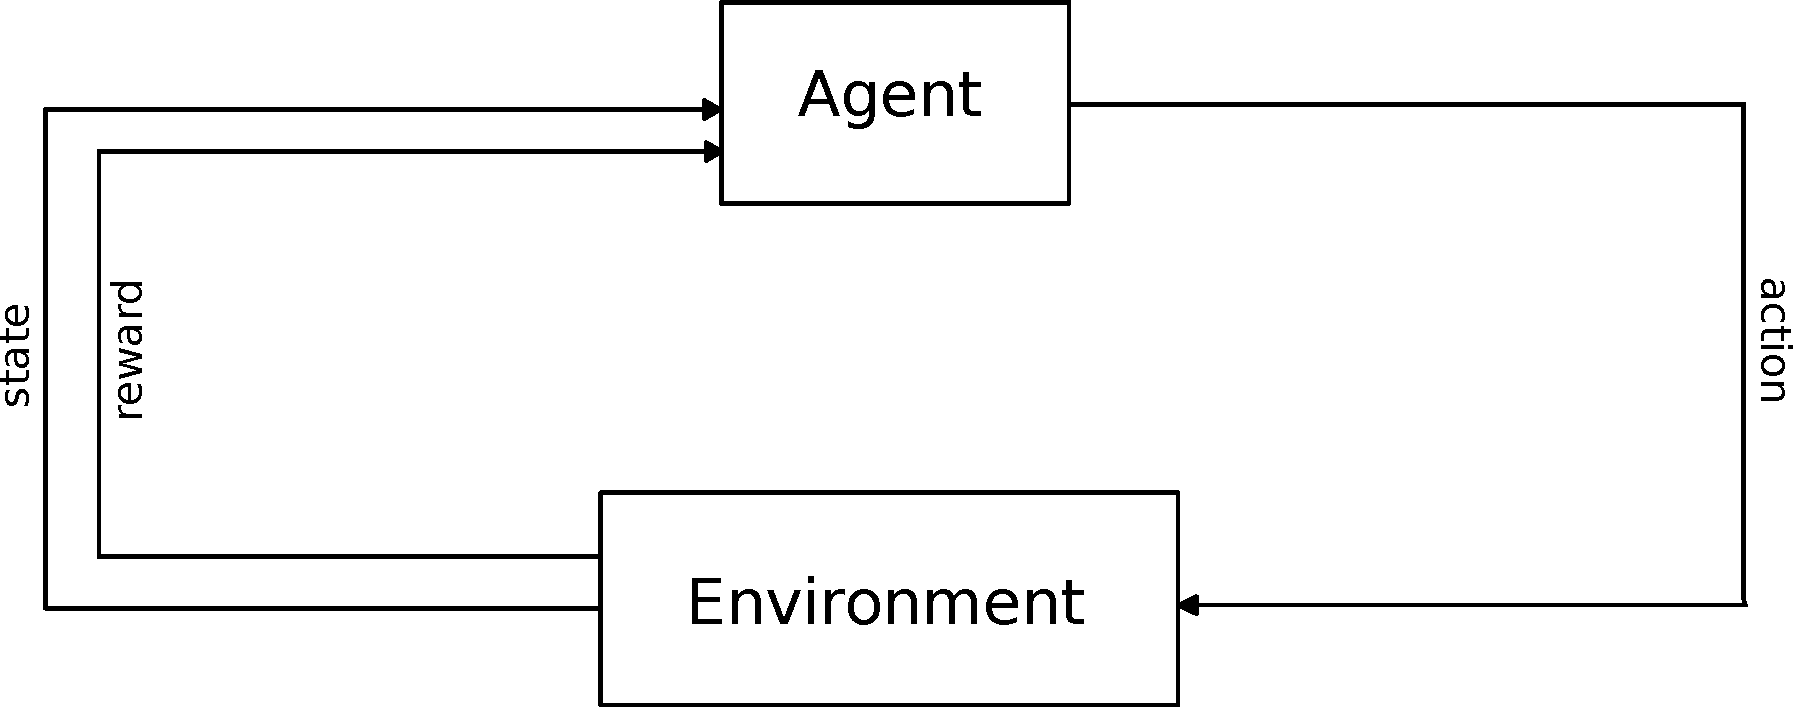
\includegraphics[scale=0.4]{pictures/rl.pdf}
	\caption{A Generic Reinforcement Learning setup}
	\label{fig:rl}
\end{figure}

\myparagraph{Multi-armed bandit} 
The setting for this study has one difference with the one of the example above. While in that case every action produces another state, and the agent will have to take another action on that state, in this study the environment reaches the terminal state after one single transition, and the agent has to choose a value for many different actions in a continuous space. 

This kind of setup is called multi-armed bandit \cite{auer2002nonstochastic}, and the main problem to solve is the balance between exploration and exploitation: we want the agent to take the best possible action, but that could prevent him to explore the environment and find even better actions.

One solution is to add simple Gaussian noise to the actions, that decays slowly as the training goes on. This way the agent is able to point in one direction, but can choose a precise value only after a high number of episodes, when he has explored the environment enough.

There are more sophisticated way to solve this problem, for example computing an estimate of the confidence on the reward obtained by taking some combination of the actions, and imposing a loss function that minimizes its values for lower values of confidence, so that the agent is ``motivated'' to explore all the action space. This kind of solution can be useful in a setup where the environment changes over time, as it is in many robotic tasks, but it could end up slowing down the training process in the simplified case of the multi-armed bandit \cite{wawrzynski2015control}.

\subsection{The simulation model} 

\myparagraph{Cortical columns}
The vast majority of cortical cortex is neocortex, the part of our brain that has developed most recently. The building blocks of neocortex are the cortical columns, defined as portions of the brain that develop perpendicular to the surface of the brain, and every column has a different receptive field from the others.

Cortical columns themselves are organized in 6 layers, that differ for cell type composition and connections with other layers and areas of the brain. Cells belongs to excitatory or inhibitory populations, and the pattern of activity that the cortical columns show, consistent between different areas and mammals \cite{kock}, is the result of the dynamical interaction of neurons in the network.

The layer 1 of the cortex is not included in the model, due to the low number of neurons contained in it, and the second and third layers are considered together, as the differences in neuron types are not considered.


\myparagraph{Integrate and fire neurons} 
Neurons are not easy to simulate, and there are models that tries to comprehend all their complexity, like Hodgkin-Huxley's, but the expense in terms of parameterization and computational weight are steep. Furthermore, in many cases, simpler neuron models like integrate and fire provide a good approximation of more complex models \cite{bernander}.  Here there is an exhaustive explanation of the integrate and fire model, which will be used in this study: 
\begin{quote}
``The integrate-and-fire neuron model is one of the most widely used models for analyzing the behavior of neural systems. It describes the membrane potential of a neuron in terms of the synaptic inputs and the injected current that it receives. An action potential (spike) is generated when the membrane potential reaches a threshold, but the actual changes associated with the membrane voltage and conductances driving the action potential do not form part of the model. The synaptic inputs to the neuron are considered to be stochastic and are described as a temporally homogeneous Poisson process.''
\begin{flushright}
\cite{burkitt}
\end{flushright}
\end{quote}



